\chapter{Dynamique}

Dans les chapitres précédents, nous avons étudié en détail différents types de
mouvements: rectiligne uniforme, rectiligne uniformément accéléré, uniformément
accéléré, circulaire uniforme et circulaire non uniforme.  Nous avons définit
quelques quantités fondamentales de la cinématique et avons déterminer des
``formules'' qui décrivent chacun des types de mouvement.  Par contre, nous
n'avons jamais déterminé quelle était la \textbf{cause} du mouvement.  C'est
ce que nous ferons dans ce chapitre-ci.

Les corps ne font pas que bouger, ils interagissent.  Ces interactions donnent
lieu à des \textbf{forces} qui elles sont responsables d'un changement dans
l'état de mouvement des corps.  Les lois de la \textbf{dynamique} décrivent
comment ces forces sont liées au mouvement, plus particulièrement à
l'accélération, des corps.

\section{La première loi de Newton}
\label{sec:La première loi de Newton}

(Section 4.1 du manuel)

Galilée a été le premier à énoncer le \textbf{principe d'inertie}.  Selon ce
principe, un objet conserve son état de mouvement si aucune force n'agit sur
lui.  Isaac Newton a formulé ce principe dans ses
\textit{Philosophi\ae~Naturalis Principia Mathematica} et l'a appelé la
\textbf{première loi} du mouvement.
\begin{marginfigure}
  \begin{center}
    \includegraphics[scale=0.38]{./04_Dynamique/newton1stlaw.png}
  \end{center}
  \caption{La première loi de Newton telle qu'elle apparaît dans les
    \textit{Principia}.}
  \label{fig:firstlaw}
\end{marginfigure}

\paragraph{Première loi de Newton}
Tout corps persévère dans son état de repos ou de mouvement uniforme en ligne
droite, sauf si des forces qui lui sont appliquées l'obligent à changer cet
état.

\paragraph{}
Dans un référentiel accéléré, la première loi de Newton n'est pas satisfaite.
Par exemple, si vous êtes dans une voiture en mouvement et que vous placez une
balle sur une surface plane devant vous, lorsque la voiture freine, la balle se
déplace vers l'avant de la voiture et semble donc subir un changement de son
état de mouvement sans qu'une force n'agisse sur elle.  Les référentiels qui
subissent une accélération sont appelés des \textbf{référentiels non-inertiels}.

Les référentiels dans lesquels la première loi de Newton est satisfaite sont
appelés des \textbf{référentiels inertiels} (Section 4.5 du manuel).  Les lois
de la physique sont plus simple à exprimer dans des référentiels inertiels et
elles ont exactement la même forme dans tous les référentiels inertiels.  Par
contre, la forme des lois de la physique peut changer lorsqu'on les exprime
dans un référentiel non-inertiel.

Puisque tout référentiel qui subit une accélération est non-inertiel, un
référentiel tournant -- par exemple, la surface de la Terre -- est un
référentiel non-inertiel.  Par contre, les accélérations en jeu ont un module
très petit, donc on peut, dans beaucoup de cas, utiliser la Terre comme une
bonne approximation d'un référentiel inertiel.

Le fait que la Terre ne soit pas un référentiel inertiel a plusieurs
conséquences intéressantes.  Par exemple, il y a une ``force'' qui pousse les
masses d'air et les nuages en mouvement dans la direction contraire au sens de
la rotation de la Terre.  Cette force fictive est appelée force de Coriolis et
elle joue un rôle important en météorologie.


\section{La force et la masse}

Si la vitesse d'un objet, disons un ourson en peluche, change, c'est parce
qu'une \textbf{force} agit sur lui.  Une force est donc une influence qui tend
à changer l'état de mouvement (i.e.: la vitesse) des corps.  Il faut cependant
faire attention: ce n'est pas parce qu'une force agit sur un corps que son
état de mouvement changera nécessairement.

Par exemple, si le professeur pousse sur l'efface à tableau, elle acquiert une
vitesse dans la même direction que la direction de la force.  Si un étudiant
pousse sur l'efface en même temps que le professeur avec une force de même
intensité, l'efface ne bouge pas, son état de mouvement reste inchangé.  De
plus, si le professeur pousse sur l'efface dans une direction différente, la
vitesse qu'elle acquiert est aussi dans cette nouvelle direction.  Par
conséquent, une \textbf{force est un vecteur} avec une norme et une
orientation.

On peut mesurer des forces en observant l'allongement d'un ressort.  Si le
professeur exerce une force sur le ressort, il s'allonge et l'allongement peut
être utilisé pour mesurer la force.  Une force deux fois plus grande causera un
allongement deux fois plus grand.

Dans le cours, nous verrons plusieurs exemples de forces.  Les plus communes
seront la tension dans une corde, la force d'un ressort, la force
gravitationnelle, la force de frottement, la force centripète.  Toutes les
forces dans la nature sont dues à quatre types d'interactions fondamentales:
l'interaction faible, l'interaction forte, l'interaction gravitationnelle et
l'interaction électromagnétique.

Si le professeur pousse sur l'efface avec une certaine force, l'efface acquiert
une certaine vitesse.  Si le professeur pousse sur un pupitre avec la même
force, le pupitre acquiert une vitesse beaucoup plus petite.  Cela est dû à la
plus grande \textbf{inertie} du pupitre.  Plus un corps a d'inertie, plus il
est difficile de modifier sont état de mouvement, c'est-à-dire qu'une force
plus grande est nécessaire pour lui faire acquérir une vitesse aussi grande que
celle de l'efface.

L'inertie est mesurée par la masse d'un objet.  Plus la masse est grande, plus
l'inertie est grande.  Ainsi, il sera plus difficile -- i.e., une force plus
grande sera requise -- de déplacer un objet plus massif qu'un objet moins
massif.

Le tableau ci-dessous résume les caractéristiques principales de la force et de
l'inertie.

\vspace{0.3cm}
\begin{fullwidth}
    \begin{tabular}{llp{8cm}l}
      \toprule
      Quantité  &  Nature   &  Description  &  Unité  \\
      \midrule
      Force     &  Vecteur  &  Influence qui tend à change la vitesse des corps  &
      newton (\si{\newton}) \\
      Masse     &  Scalaire &  Mesure de l'inertie, i.e., de la résistance aux
      variations de vitesse; propriété intrinsèque  &  kilogramme (\si{\kilo\gram}) \\
      \bottomrule
    \end{tabular}
\end{fullwidth}
\vspace{0.3cm}

Dans le cours, il sera souvent utile de faire la distinction entre une
\textbf{force de contact} et une \textbf{force à distance}.  Une force de
contact s'exerce quand deux objets sont en contact physique l'un avec l'autre.
Par exemple, lorsque le professeur pousse sur l'efface, il y a un contact
direct entre la main du professeur et l'efface.  De même, si une corde est
attachée à un bloc et qu'on tire sur la corde, au point de contact de la corde
et du bloc, une force s'exerce sur le bloc.  Les forces à distance agissent
entre deux objets sans qu'un milieu matériel entre les deux ne soit nécessaire.
La force de gravité entre la Terre et le Soleil, et la force électrique entre
un électron et un proton sont deux exemples de forces à distance.

Il est important de réaliser que cette distinction n'a de sens que dans un
contexte macroscopique, c'est-à-dire à grande échelle.  À l'échelle
microscopique, toutes les forces sont des forces à distance et la distinction
devient tout à fait artificielle.


\section{La force nette}

Il est possible qu'une force agisse sur un corps mais que sa vitesse ne varie
pas.  Par exemple, si le professeur pousse l'efface vers la droite et qu'un
étudiant pousse l'efface vers la gauche avec la même intensité -- i.e., forces
de même module -- alors l'efface ne bouge pas, sa vitesse demeure inchangée.
L'état de mouvement d'un corps ne change que si la \textbf{force
nette}, c'est-à-dire la somme vectorielle de toutes les forces, est non nulle.

\paragraph{Exemple -- Force nette}

On considère une boîte de pizza qu'essaient de s'arracher trois personnes tel
qu'indiqué dans la figure ci-contre.  Le module de la force exercée par Han est
de \SI{9}{\newton}, celui de la force exercée par Leia est de \SI{4}{\newton},
et celui de la force exercée par Luke est \SI{8}{\newton}.

\begin{marginfigure}
  \begin{center}
  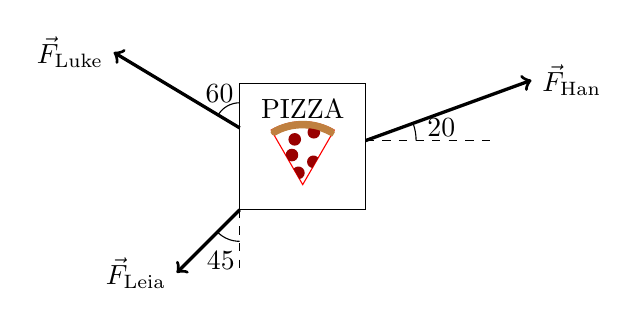
\begin{tikzpicture}[scale=0.8]
    \draw (-1, -1) rectangle (1, 1);
    \begin{scope}[shift={(0, -0.6)}]
      \draw[red] (0, 0) -- ++(60:1) arc (60:120:1) -- cycle;
      \filldraw[brown, rounded corners=0.7] (59:0.9) -- (59:1)
        arc (59:121:1) -- (121:0.9) arc (121:59:0.9);
      \clip (0, 0) -- ++(60:0.9) arc (60:120:0.9) -- cycle;
      \fill[red!60!black] (65:0.4) circle (0.1);
      \fill[red!60!black] (100:0.73) circle (0.1);
      \fill[red!60!black] (78:0.85) circle (0.1);
      \fill[red!60!black] (110:0.5) circle (0.1);
      \fill[red!60!black] (110:0.2) circle (0.1);
    \end{scope}
    \node at (0, 0.6) {PIZZA};
    \draw[very thick, ->] (-1, 0.3) -- (-3, 1.5) node[left] {$\vec{F}_\mathrm{Luke}$};
    \draw (-1, 0.7) arc (90:150:0.4);
    \node at (-1.32, 0.85) {\SI{60}{\degree}};
    \draw[very thick, ->] (-1, -1) -- (-2, -2) node[left] {$\vec{F}_\mathrm{Leia}$};
    \draw[dashed] (-1, -1) -- (-1, -2);
    \draw (-1, -1.5) arc (-90:-135:0.5);
    \node at (-1.3, -1.8) {\SI{45}{\degree}};
    \draw[very thick, ->] (1, 0.1) -- ++(20:2.8) node[right] {$\vec{F}_\mathrm{Han}$};
    \draw[dashed] (1, 0.1) -- (3, 0.1);
    \draw (1.8, 0.1) arc (0:20:0.8);
    \node at (2.2, 0.3) {\SI{20}{\degree}};
  \end{tikzpicture}
  \end{center}
\end{marginfigure}

Déterminer la force nette qui agit sur la boîte de pizza.

\begin{marginfigure}
  \begin{center}
  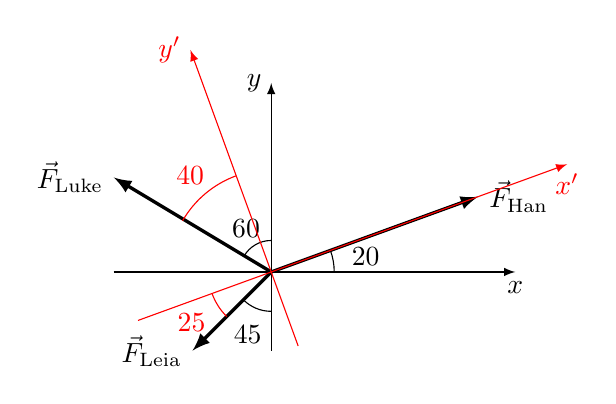
\begin{tikzpicture}[>=latex]
    \draw[->] (0, -1) -- (0, 2.4) node[left] {$y$};
    \draw[->] (-2, 0) -- (3.1, 0) node[below] {$x$};
    \begin{scope}[shift={(1, -0.3)}]
      \draw[very thick, ->] (-1, 0.3) -- (-3, 1.5) node[left] {$\vec{F}_\mathrm{Luke}$};
      \draw (-1, 0.7) arc (90:150:0.4);
      \node at (-1.32, 0.85) {\SI{60}{\degree}};
    \end{scope}
    \begin{scope}[shift={(1, 1)}]
      \draw[very thick, ->] (-1, -1) -- (-2, -2) node[left] {$\vec{F}_\mathrm{Leia}$};
      \draw (-1, -1.5) arc (-90:-135:0.5);
      \node at (-1.3, -1.8) {\SI{45}{\degree}};
    \end{scope}
    \begin{scope}[shift={(-1, -0.1)}]
      \draw[very thick, ->] (1, 0.1) -- ++(20:2.8) node[right] {$\vec{F}_\mathrm{Han}$};
      \draw (1.8, 0.1) arc (0:20:0.8);
      \node at (2.2, 0.3) {\SI{20}{\degree}};
    \end{scope}
    \draw[red, ->] (200:1.8) -- (20:4) node[below] {$x'$};
    \draw[red, ->] (-70:1) -- (110:3) node[left] {$y'$};
    \draw[red] (110:1.3) arc (110:150:1.3);
    \node[red] at (130:1.6) {\SI{40}{\degree}};
    \draw[red] (200:0.8) arc (200:225:0.8);
    \node[red] at (212.5:1.2) {\SI{25}{\degree}};
  \end{tikzpicture}
  \end{center}
\end{marginfigure}

La première chose à faire est de faire un schéma simplifié de la situation dans
lequel on précise le système d'axes qu'on va utiliser.  Dans ce cas-ci, le
système ``habituel'' n'est pas le plus simple à utiliser.  Le calcul sera plus
facile si on prend un système d'axes dans lequel au moins une des forces est
orientée le long d'un axe.

Dans le système d'axe en rouge:
\begin{align*}
  \vec{F}_\mathrm{Han} &= \SI{9}{\newton}\xhat \\
  \vec{F}_\mathrm{Luke} &= \left(-\num{8} \sin \SI{40}{\degree} \xhat
                           + \num{8} \cos \SI{40}{\degree} \yhat \right) \si{\newton}\\
  \vec{F}_\mathrm{Han} &=  \left(-\num{4} \cos \SI{25}{\degree} \xhat
                           - \num{4} \sin \SI{25}{\degree} \yhat \right)
                         \si{\newton} \\
\end{align*}

La force nette est la somme vectorielle de ces trois forces.  Par
conséquent:
\begin{align*}
  \vF &= \vF_\mathrm{Han} + \vF_\mathrm{Luke} + \vF_\mathrm{Leia}  \\
      &= \left(9 -\num{8} \sin \SI{40}{\degree} -\num{4} \cos \SI{25}{\degree} \right) \xhat \si{N}
        +\left( \num{8} \cos \SI{40}{\degree} - \num{4} \sin \SI{25}{\degree}
        \right)\yhat \si{N}
\end{align*}
\[
  \boxed{\vF = \left( \num{0.232}\xhat + \num{4.44}\yhat \right) \si{N}}
\]


\section{La deuxième loi de Newton}

Jusqu'ici nous avons défini la force, la masse, l'inertie, et nous avons énoncé
la première loi de Newton.  Si une force unique agit sur un corps d'une
certaine masse, la force a tendance à modifier la vitesse de ce corps dans la
direction de la force.  Plus le corps possède d'inertie, plus le changement de
vitesse sera petit.  Autrement dit, le changement de vitesse est proportionnel
à la force et inversement proportionnel à l'inertie.
\[
  \Delta \vv \propto \frac{\vF}{\mathrm{inertie}} 
\]
Or, le changement de vitesse est proportionnel à l'accélération et l'inertie
est donnée la masse du corps, donc
\[
  \va \propto \frac{\vF}{m}
\]
De nombreuses expériences en laboratoire on permis de valider que la relation
est une égalité stricte.  On obtient la deuxième loi de Newton.
\begin{marginfigure}
  \begin{center}
    \includegraphics[scale=0.38]{./04_Dynamique/newton2ndlaw.png}
  \end{center}
  \caption{La première loi de Newton telle qu'elle apparaît dans les
    \textit{Principia}.}
  \label{fig:firstlaw}
\end{marginfigure}

\[
  \vec{F} = m\vec{a}
\]

Lorsque plusieurs forces agissent sur un même corps, alors c'est la force nette
qui détermine l'accélération du corps.
\[
  \boxed{\vF_\mathrm{nette} = \sum \vF = m\va}
\]

\begin{itemize}
  \item Une force \textbf{cause} un changement de vitesse.
  \item L'accélération est l'\textbf{effet} ou la \textbf{conséquence} de la force.
  \item L'accélération est dans la même direction que la force nette.
  \item Si une force nette agit sur un corps, alors ce corps subira une accélération.
  \item Si un corps subit une accélération, c'est parce qu'une force nette agit sur lui.
  \item Si un corps est au repos ou en mouvement rectiligne à vitesse
    constante, il ne subit aucune force et la force nette sur le corps est donc
    nulle.
  \item Une même force qui agit sur deux corps différents n'aura pas
    nécessairement le même effet (ie, le corps n'accélérera pas de la même
    façon) parce que les masses des deux corps ne sont pas forcément
    identiques.
\end{itemize}


\section{La troisième loi de Newton}

Pour toute force exercée par un corps $A$ sur un corps $B$, le corps $B$ exerce
une force de module égal et de direction opposée sur $A$:
\[
  \vF_{AB} = -\vF_{BA}
\]



\section{La loi de la gravitation universelle}

Newton, en plus de découvrir ses trois lois du mouvement, énonça une loi
universelle de la gravitation.  L'attraction gravitationnelle entre deux corps
est proportionnelle à la masse de chacun des corps et inversement
proportionnelle au carré de la distance qui les sépare.  C'est une force
attractive qui est orientée le long de l'axe reliant les deux corps.
\[
  \vF_g = \frac{Gm_1m_2}{r^2} \vec{u}_r
\]
où $G$ est la constante de la gravitation $G = \SI{6.672e-11}{Nm^2/kg^2}$.
